\section{eo\-PBILDistrib$<$ EOT $>$ Class Template Reference}
\label{classeo_p_b_i_l_distrib}\index{eoPBILDistrib@{eoPBILDistrib}}
Distribution Class for PBIL algorithm (Population-Based Incremental Learning, Baluja and Caruana 96).  


{\tt \#include $<$eo\-PBILDistrib.h$>$}

Inheritance diagram for eo\-PBILDistrib$<$ EOT $>$::\begin{figure}[H]
\begin{center}
\leavevmode
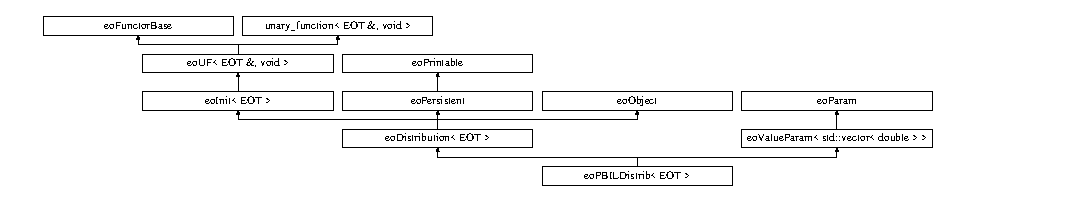
\includegraphics[height=2.26721cm]{classeo_p_b_i_l_distrib}
\end{center}
\end{figure}
\subsection*{Public Member Functions}
\begin{CompactItemize}
\item 
{\bf eo\-PBILDistrib} (unsigned \_\-genome\-Size)\label{classeo_p_b_i_l_distrib_a0}

\begin{CompactList}\small\item\em Ctor with size of genomes, and update parameters. \item\end{CompactList}\item 
virtual void {\bf operator()} ({\bf EOT} \&\_\-eo)\label{classeo_p_b_i_l_distrib_a1}

\begin{CompactList}\small\item\em the randomizer of indis \item\end{CompactList}\item 
unsigned {\bf Size} ()\label{classeo_p_b_i_l_distrib_a2}

\begin{CompactList}\small\item\em Accessor to the genome size. \item\end{CompactList}\item 
virtual void {\bf print\-On} (std::ostream \&os) const \label{classeo_p_b_i_l_distrib_a3}

\begin{CompactList}\small\item\em printing... \item\end{CompactList}\item 
virtual void {\bf read\-From} (std::istream \&is)\label{classeo_p_b_i_l_distrib_a4}

\begin{CompactList}\small\item\em reading... \item\end{CompactList}\item 
unsigned int {\bf size} ()\label{classeo_p_b_i_l_distrib_a5}

\item 
virtual std::string {\bf class\-Name} () const 
\begin{CompactList}\small\item\em class\-Name: Mandatory because of {\bf eo\-Combined\-Init}{\rm (p.\,\pageref{classeo_combined_init})}. \item\end{CompactList}\end{CompactItemize}
\subsection*{Private Attributes}
\begin{CompactItemize}
\item 
unsigned {\bf genome\-Size}\label{classeo_p_b_i_l_distrib_r0}

\end{CompactItemize}


\subsection{Detailed Description}
\subsubsection*{template$<$class EOT$>$ class eo\-PBILDistrib$<$ EOT $>$}

Distribution Class for PBIL algorithm (Population-Based Incremental Learning, Baluja and Caruana 96). 

It encodes a univariate distribution on the space of bitstrings, i.e. one probability for each bit to be one

It is an {\bf eo\-Value\-Param}{\rm (p.\,\pageref{classeo_value_param})}$<$std::vector$<$double$>$ $>$ : the std::vector$<$double$>$ stores the probabilities that each bit is 1

It is still pure virtual, as the update method needs to be specified 



Definition at line 44 of file eo\-PBILDistrib.h.

\subsection{Member Function Documentation}
\index{eoPBILDistrib@{eo\-PBILDistrib}!className@{className}}
\index{className@{className}!eoPBILDistrib@{eo\-PBILDistrib}}
\subsubsection{\setlength{\rightskip}{0pt plus 5cm}template$<$class EOT$>$ virtual std::string {\bf eo\-PBILDistrib}$<$ {\bf EOT} $>$::class\-Name (void) const\hspace{0.3cm}{\tt  [inline, virtual]}}\label{classeo_p_b_i_l_distrib_a6}


class\-Name: Mandatory because of {\bf eo\-Combined\-Init}{\rm (p.\,\pageref{classeo_combined_init})}. 

SHould be pure virtual, but then we should go over the whole code to write the method for all derived classes ... MS 16/7/04 

Reimplemented from {\bf eo\-Init$<$ EOT $>$} {\rm (p.\,\pageref{classeo_init_a0})}.

Definition at line 94 of file eo\-PBILDistrib.h.

The documentation for this class was generated from the following file:\begin{CompactItemize}
\item 
eo\-PBILDistrib.h\end{CompactItemize}
